\documentclass[a4paper, 10pt]{article}
\usepackage{graphicx}
\usepackage[margin = 1in]{geometry}
\usepackage{parskip}
\usepackage[hidelinks, colorlinks = true, citecolor = black, linkcolor = blue]{hyperref}
\usepackage{amsmath}
\usepackage{tabularx}
\usepackage{csvsimple}
\usepackage{ragged2e}
\usepackage{cite}
\usepackage{pdfpages}
\usepackage{subcaption}
\newcommand{\inv}{^{\raisebox{.2ex}{$\scriptscriptstyle-1$}}}
\newcommand{\unit}[1]{~\mathrm{#1}}

\begin{document}
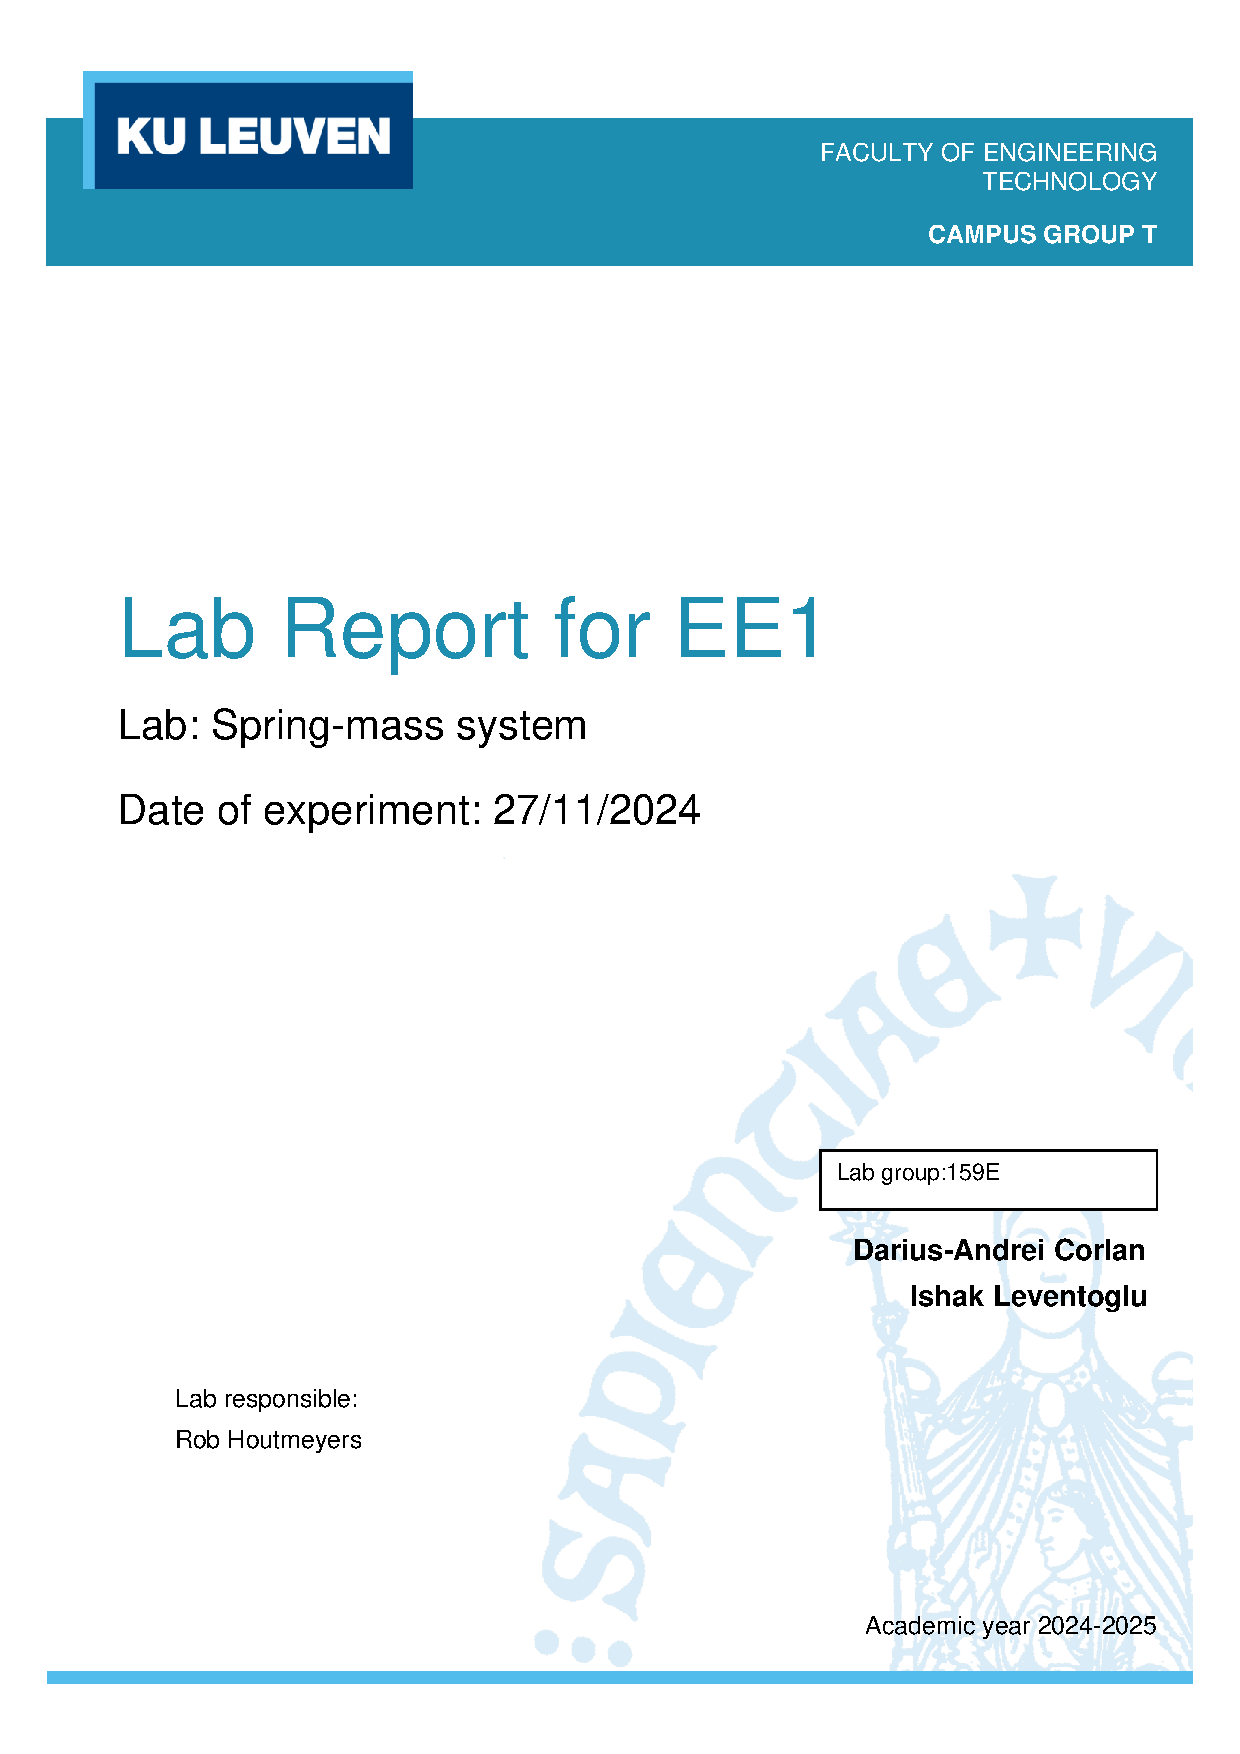
\includepdf[pages = {1}]{template.pdf}
\begin{justify}
\section{Introduction}
The aim of this lab is to measure the spring constant of a helical spring and to
compare it to the theoretical value. Afterwards, the period of vibration will also be
measured, while also measuring the effect of spring mass on this value.
\section{Theory}
Hooke's law, as defined by the 17th century physicist Robert Hooke, states that
the force exerted by a spring is directly proportional to the elongation or
compression of the spring\cite{williams_what_nodate}.
\par
A helical spring is a part of wire coiled or wound in the shape of a helix. When
a spring with the spring constant $k$ and the unstretched length $l_0$ is
stretched or compressed to the length $l_e$, the force exerted by the spring
will be a relation between $k$ and $\Delta l$. For small deflections Hooke's law
is formulated in Equation 1\cite{williams_what_nodate}.
%refr
\par
\begin{equation}
    F_e = -kx = -k(l_e - l_0)
\end{equation}
Where:
\begin{itemize}
    \item $F_e$ is the force exerted by the spring
    \item $k$ is the spring constant
    \item $x$ is the displacement
    \item $l_e$ is the stretched length of the spring
    \item $l_0$ is the unstretched length of the spring
\end{itemize}
Considering an ideal spring, we mount a system made of a helical spring and a
mass at the end vertically, where it gets to an equilibrium position. The force
of the spring in the equilibrium position is equal to the weight force of the
object.
\par
\begin{equation}  \label{eq:2}
    k x_e = mg 
\end{equation}
When displacing the mass from the equilibrium position, the system will start
oscillating.
Using Newton's second law, Equation 3 is determined.
\begin{align} 
    m \frac{d^2 x}{d t^2} &= mg - kx = mg - k (x_e + x^{\prime}) \\
\intertext{Since:} \nonumber \\   
    k x_e &= Cst \nonumber \\ 
    \frac{d^{\,2} x}{d t^2} &= \frac{d^2 x^{\prime}}{d t^2} \text{($x_e$ is constant, $x = x_e + x^\prime$)} \nonumber
\intertext{The equation becomes:} \nonumber \\
    \frac{d^{\,2} x^{\prime}}{d t^2} &= -\frac{k}{m}x^{\prime} \label{eq:4}
\end{align}
Where $x^{\prime}$ is the position relative to the equilibrium position.
\newpage
Solving the differential equation, Equation~\ref{eq:4} an expression for the relative
position is found:
\begin{equation}
    x^{\prime}(t) = Acos(\sqrt{\frac{k}{m}}t + \Phi)
\end{equation}
Where:
\begin{itemize}
    \item $x^{\prime}(t)$ is the position relative to the equilibrium position
    \item $A$ is the amplitude
    \item $\Phi$ is the phase angle~(constant value that depends on initial conditions)
\end{itemize}
\par
The time period is given by Equation~\ref{eq:6}:
\begin{equation} \label{eq:6}
    T_{id} = 2 \pi \sqrt{\frac{m}{k}}
\end{equation}
However, since the impact of the spring's weight cannot be ignored, the formulas
have to be modified to include the moment of inertia, which affects k. To
account for this, the corrected formula is used:
\begin{equation} \label{eq:7}
    T_{cor} = 2 \pi \sqrt{\frac{m+\frac{m_S}{3}}{k}}
\end{equation}
These formulas are used to validate Hooke's law and determine the spring
constant. The corrected formula for period can also be used to compare
measurements to theoretical values.
\section{Method and Materials}
\subsection{Experimental setup}
The setup for the experiment consists of a spring mounted to a vertical stand
and a ruler next to the spring. Weight is added progressively, changing
displacements to accurately calculate the spring constant. The mass is measured
using a digital scale, displacement is measured with a ruler and the period is
measured using a chronometer. Figure 1 shows the experimental setup.
\begin{figure}[!h]
    \centering
    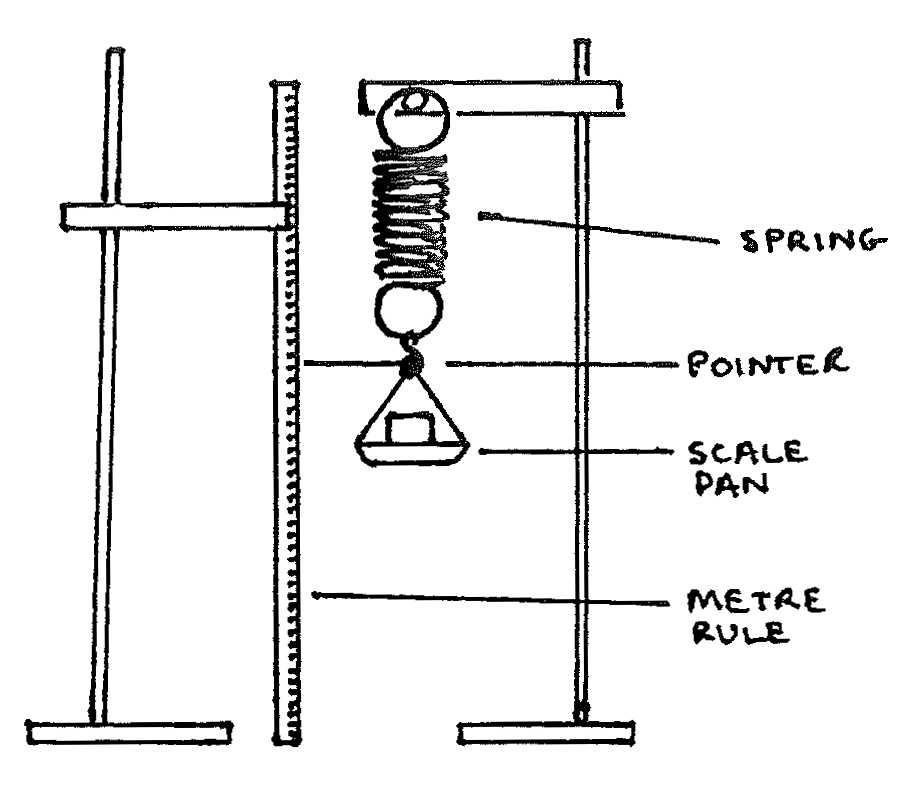
\includegraphics[width = 0.5\linewidth]{13.png}
    \caption{Drawing of the experiment setup\cite{noauthor_b5-2_nodate}}
\end{figure}
\newpage
\subsection{Measuring instruments}
\begin{itemize}
    \item Vertical meter ruler with 1mm increment ($\pm 0.5\unit{mm}$ uncertainty)
    \item Digital scale ($\pm 0.01\unit{g}$ uncertainty)
    \item Helical spring
    \item Smartphone used as chronometer ($\pm  0.01\unit{s} $)
    \item Spring stand
\end{itemize}
\subsection{Method}
\justifying
For the first experiment, the spring is attached to the vertical stand with a ruler by its side. Weights
with known mass are added to the spring, measuring the elongation which are used
to calculate the spring constant $k$.
\par
For the second experiment, weights are attached to the spring, the weights
are displaced and the time for 30 oscillations to happen is measured three
times. By repeating the experiment with multiple masses, the theoretical values
can be more accurately compared to the experimental results.
\section{Results spring constant}
\subsection{Measurements}
The measured values for the mass of the holder plus discs $m$, the unstretched
length $l_0$, the stretched length $l_1$, the elongation $x_e$ and the spring
constant $k$ for both the short and long spring are described in tables 1 and 2.
\begin{table}[!h]
    \centering
    \caption{Measurements for the short spring}
    \label{tab:1}
    \begin{tabular}{|c|c|c|c|c|c|c|} 
    \hline
    mass of discs [g] & $l_0$ [cm] & $l_1$ [cm] & $x_e$ [m] &
    $mg$ [N]  & $k$ [$\mathrm{Nm\inv}$] & $\Delta k$ [$\mathrm{Nm\inv}$]  \\ 
    \hline
    31.1                              & 4.7     & 13.1    & 0.08   & 0.31 & 3.63     & 0.16    \\ 
    \hline
    52.1                              & 4.7     & 18.5    & 0.14   & 0.51 & 3.70     & 0.10    \\ 
    \hline
    70.8                               & 4.7     & 24.4    & 0.20   & 0.69 & 3.53     & 0.07    \\ 
    \hline
    91.9                               & 4.7     & 29.95   & 0.25  & 0.90 & 3.57     & 0.05   \\ 
    \hline
    110.46                             & 4.7     & 35.4    & 0.31   & 1.08 & 3.53     & 0.05     \\
    \hline
    \end{tabular}
\end{table}
\begin{table}[!h]
    \centering
    \caption{Measurements for the long spring}
    \begin{tabular}{|c|c|c|c|c|c|c|} 
    \hline
    mass of the discs [g] & $l_0$ [cm] & $l_1$ [cm] & $x_e$ [m] & $mg$ [N]  &
    $k$ [$\mathrm{Nm\inv}$] & $\Delta k$ [$\mathrm{Nm     \inv}$]        \\ 
    \hline
    31.14                 & 17.35   & 18.7    & 0.014 & 0.31 & 22.63      & 5.93  \\ 
    \hline
    52.14                 & 17.35   & 19.7    & 0.024 & 0.51 & 21.77     & 3.27 \\ 
    \hline
    70.8                  & 17.35   & 20.65   & 0.033  & 0.69 & 21.05     & 2.26  \\ 
    \hline
    91.9                  & 17.35   & 21.6    & 0.043 & 0.90 & 21.21     & 1.77  \\ 
    \hline
    110.46                & 17.35   & 22.7    & 0.054 & 1.08 & 20.25     & 1.34  \\
    \hline
    \end{tabular}
\end{table}
\newpage
\subsection{Graphs}
By plotting the values in Tables 1 and 2, the spring constant of each spring can
be determined. A graph for each spring, with the weight as a function of elongation is plotted,
is shown in Figures 2 and 3.
\begin{figure}[!h]
    \centering
    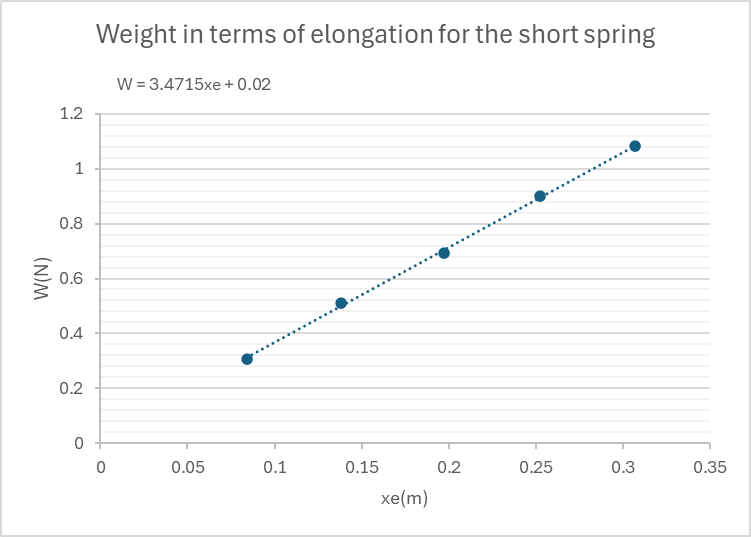
\includegraphics[width = 0.7\linewidth]{constant_short_spring.png}
    \caption{Weight as a function of elongation for the short spring}
    \label{fig:2}
\end{figure}
\begin{figure}[!h]
    \centering
    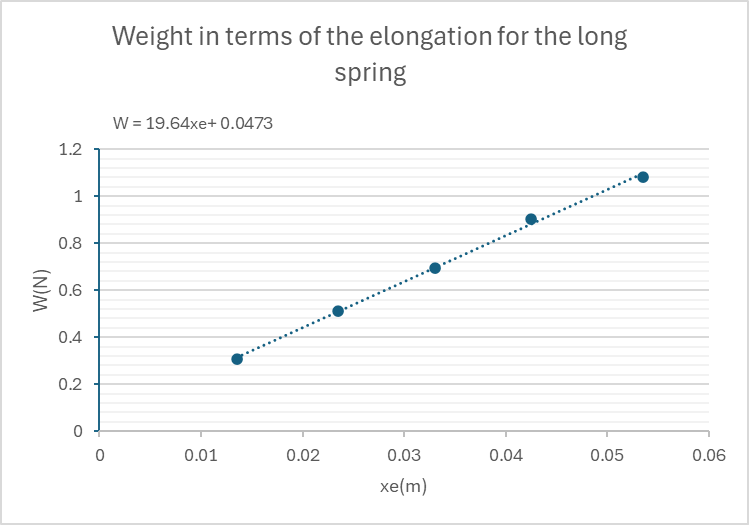
\includegraphics[width = 0.7\linewidth]{constant_long_spring.png}
    \caption{Weight as a function of elongation for the long spring}
    \label{fig:3}
\end{figure}
\subsection{Calculations}
Using the measured values, the spring constants can be determined. To determine
$x_e$ the following equation is used:
\begin{equation}
    x_e = l_1 - l_0
\end{equation}
To calculate the force that is applied to the spring, the weight equation is
used:
\begin{equation}
    W = mg
\end{equation}
By using equation \ref{eq:2} the spring constant can be therefore calculated.
\subsubsection{Example calucaltion}
By using the fifth data point of table \ref{tab:1}, the following calculations
are made to determine the spring constant.
\begin{gather*}
\intertext{Firstly, the weight of the discs and hook are calculated:} \\
 W = m \cdot g = 110.46\unit{g} \cdot 0.001\unit{\frac{g}{kg}} \cdot 9.81\unit{\frac{kg}{N}} = 1.0836\unit{N} \approx 1.08\unit{N}\\
\intertext{Afterwards, the elongation is calculated:} \\
 x_e = l_1 - l_0 = 35.4\unit{cm} - 4.7\unit{cm} = 30.7\unit{cm} \approx 0.31\unit{m}\\
\intertext{Finally, the spring constant can be calculated using equation \ref{eq:2}:} \\
k x_e = W \Rightarrow k = \frac{W}{x_e} = \frac{1.0836 \unit{N}}{0.31\unit{m}} = 3.5296\unit{Nm\inv} \approx 3.53\unit{Nm\inv} 
\end{gather*}
\subsubsection{Error calculations}
As the mass was calculated using a digital scale, the uncertainty is the sum of
the smallest division\cite{profcomp}.
\[ \Delta m = 0.01\unit{g} = 0.01\unit{g} \cdot 10^{-3}\unit{kg}\]
Since both $l_0$ and $l_1$ were measured using two markers on a ruler, the
uncertainty in the measurement is equal to half of the smallest division\cite{profcomp}.
\[ \Delta l_0 = \Delta l_1 = \frac{0.05\unit{cm}}{2} = 0.025\unit{cm} =
0.025 \cdot 10^{-2}\unit{m} \]
The error of the extension is calculated by propagating the error of the
measurements \cite{profcomp}:
\[ \Delta x_e = \sqrt{\Delta l_0 ^{\,2} + \Delta l_1 ^{\,2}} =
\sqrt{(0.025\unit{cm})^2 + (0.025\unit{cm})^2} = 0.03535\unit{cm}
\approx 0.04 \cdot 10^{-2}\unit{m}\]
For the weight, the error is calculated by multiplying the error of the mass
with the constant, $g$:
\[\Delta W = \Delta m |g| = (0.01 \cdot 10^{-3}\unit{kg})|9.81~
\mathrm{kg \cdot N\inv}| = 9.81 \cdot 10^{-5}\unit{N}\]
To calculate the error of the spring constant, the following equation is used \cite{profcomp}:
\begin{equation}\label{eq:10}
    \Delta k = |k|\sqrt{\left(\frac{\Delta W}{|W|}\right)^2 + \left( \frac{\Delta x_e}{|x_e|}\right) ^2}
\end{equation}
By using the fifth data point of table \ref{tab:1}, we get the error for the
spring constant:
\[ \Delta k = \left| k \right| = \sqrt{\left(\frac{9.81 \cdot 10
^{-5}\unit{N}}{1.083}\right) ^ 2 + \left(\frac{0.04 \cdot 10^
{-2}\unit{m}}{0.314\unit{m}}\right) ^ 2 } = 0.04065 \unit{N m\inv}
\approx 0.05\unit{N m\inv}\]
\newpage
\textbf{Calculating the spring error and constant:}
\par
The average spring constant is calculated using the arithmetic mean:
\begin{equation}
    k_{avg} = \frac{1}{n} \sum_{i=1}^{n} k_i
\end{equation}
The example calculation for the short spring is:
\[k_{avg}  = \frac{1}{5}\left(3.63\unit{N m\inv}+ 3.70\unit{N m\inv} +
3.52\unit{N m\inv} + 3.57\unit{N m\inv} + 3.52\unit{N m\inv} \right)  =
3.5\unit{N m\inv}\]
The error of the average spring constant is calculated using the standard
deviation of the mean \cite{profcomp}:
\begin{equation}\label{eq:12}
s_m = \frac{s}{\sqrt{n}}
\end{equation}
Where n is the number of samples and s is the standard deviation, defined
as \cite{profcomp}:
\begin{equation}\label{eq:13}
s = \sqrt{\frac{\sum_{i=1}^{n}(k_i-k_{avg})^2}{n-1}}
\end{equation}
To obtain $\Delta k_{avr}$, $s_m$ is multiplied by a constant, $t$, which in
this case is 3 \cite{profcomp}:
\begin{equation}\label{eq:14}
    \Delta k_{avg} = 3s_m
\end{equation}
When substituting values for the short spring, the results are:
\begin{gather*}
    s = 0.077\unit{N m\inv}\\
    s_m = 0.035\unit{N m\inv}\\
    \Delta k_{avr} = 0.105\unit{N m\inv}
\end{gather*}
The results for the long spring:
\begin{gather*}
    s = 0.8814\unit{N m\inv}\\
    s_m = 0.3945\unit{N m\inv}\\
    \Delta k_{avr} = 1.1835\unit{Nm\inv}
\end{gather*}
Therefore,
\[ k_{s_{avg}} = (3.5 \pm 0.2)\unit{Nm\inv}\]
\[k_{l_{avg}} = (21.38 \pm 1.19)\unit{Nm\inv}\]
\par
\textbf{From the graphs}
\par
The value of the spring constant can also be determined from the trendline of
the graphs in figures \ref{fig:2} and \ref{fig:3}.
\par
Therefore, figure \ref{fig:2} and \ref{fig:3} can be interpreted so that the
average spring constants can be found.
\begin{gather*}
 k_{s_{avg}} = 3.741\unit{Nm\inv}\\
 k_{l_{avg}} = 19.64\unit{Nm\inv}
\end{gather*}
\newpage
\section{Discussion spring constant}
\justifying
The purpose of this experiment was to evaluate the accuracy and precision of the measurements as well as the link between the physical quantities involved, such as force and extension in the context of Hooke's Law. The project accomplished its goal, albeit with certain restrictions, according to the data gathered and analyzed.
\par
The method used to take measurements using the ruler was one of the primary causes of inaccuracy. The readings might have been impacted by parallax inaccuracies if the spring wasn't vertical or the ruler wasn't precisely positioned at eye level. There was also some variance because the spring wasn't always perfectly still when measurements were made. The greatest measurement uncertainty was introduced by using a manual ruler as opposed to instruments such as a digital displacement sensor. The slight variations between the expected and observed outcomes can be explained by these problems.
\par
Despite minor departures from the theoretical predictions, the final results fell within the allowable error range. The spring constant (k), for example, was represented by the force-extension graph, whose slope was near the expected value but had variations just outside the anticipated error ranges. The previously noted measurement inaccuracies are probably the cause of these variances.
\par
Although there were a few minor differences, there was generally agreement when comparing the results with those of other organizations carrying out the same experiment. The observed changes were marginally more noticeable than values from earlier research, suggesting that the techniques employed could be improved.
\par
It was discovered that the force-extension connection was linear, in accordance
with Hooke's Law. The spring constant (k), represented by the graph's slope, was
determined to be (value), falling within (percentage)\% of the theoretical
value. As anticipated for minor deformations, this validated the
force-displacement proportionality.
\par
A few adjustments could be made to future studies to increase accuracy. Precision would be increased and parallax errors would be eliminated with the use of a digital measurement equipment. Inconsistencies would also be decreased by stabilizing the spring prior to collecting measurements. The effect of random errors would be reduced by doing measurements several times and averaging them. More dependable results could also be obtained by fixing the ruler so that it is exactly perpendicular to the spring.
\subsection{Specific questions}
Does the spring comply with Hooke's law? Explain!
\par
In the context of this experiment, the spring does, in fact, adhere to Hooke's law. The spring's extension is proportionate to the applied force, as indicated by the force-extension graph's obvious linear relationship. Hooke's law predicts just this. The notion that no force implies no expansion is further supported by the line's proximity to the origin. Although we didn't push the spring that far in this experiment, deviations may occur if we used considerably greater forces since the spring could approach its elastic limit.
\par
What is your best value of k?
\par
The graph's slope was used to determine the ideal value of k, the spring constant. The data showed that (value with units) was the result. This number, which represents the spring's stiffness, remained largely constant across the many measurements we made.
\par
Does the average value from the table correspond to the value from the graph
within the measurement error?
\par
Indeed, within the anticipated measurement error, the average value of k from the table and the value we obtained from the graph agree. Any slight discrepancies are probably the result of small problems, such as a tiny parallax mistake in the ruler's reading or tiny spring movements prior to the measurements. Overall, there is good agreement between the two values.
\section{Results period experiment}
\subsection{Measurements}
The measurements of the period, by counting 30 oscillations of mass $m$, are
presented in table 3 and 4. Included in these tables are also the values for the
average period of oscillation of each mass, $T_{ex}$, the ideal period, $T_{id}$,
and the theoretical period using the corrected mass $T_{cor}$. The percent
deviation between the ideal and experimental values of both $T_{id}$ and
$T_{cor}$ are included. For the long spring, as it was not possible to stop the
spring from behaving like a pendulum, a smaller number of oscillations had to be
measured, marked in table 4.
\begin{table}[!h]
    \centering
    \caption{Measurement results for the second experiment when using the short spring}
    \label{tab:3}
    \begin{tabular}{|c|c|c|c|c|c|c|c|c|} 
    \hline
     $m~[10^{-3} \unit{kg}]$ & $30 T_1$  & $30 T_2$  & $30 T_3$  & $T_{ex}~[\mathrm{s}]$    & $T_{id} \unit{[s]}$     & $T_{cor} \unit{[s]}$    & $PD_{id} \unit{[\%]}$ & $PD_{cor} \unit{[\%]}$  \\ 
    \hline
    31.14            & 18.78 & 19.09 & 18.9  & 0.63 & 0.58 & 0.68 & 7.32  & 7.01    \\ 
    \hline
    52.14            & 23.57 & 23.59 & 23.72 & 0.79 & 0.76 & 0.87 & 3.95  & 10.91    \\ 
    \hline
    70.8             & 27.51 & 27.34 & 27.19 & 0.91 & 0.88 & 1.02 & 3.30  & 11.66    \\ 
    \hline
    91.9             & 30.82 & 30.92 & 30.7  & 1.03 & 1.01 & 1.16 & 2.23 & 12.90    \\
    \hline
    \end{tabular}
\end{table}
\begin{table}[!h]
    \centering
    \caption{Measurement results for the second experiment using the long spring}
    \begin{tabular}{|c|c|c|c|c|c|c|c|c|} 
        \hline
        $m~[10^{-3}\unit{kg}]$ & $30 T_1$ & $30 T_2$  & $30 T_3$  & $T_{ex} \unit{[s]}$    & $T_{id} \unit{[s]}$     & $T_{cor} \unit{[s]}$    & $PE_{id}\unit{[\%]}$     & $PE_{cor}\unit{[\%]}$     \\ 
        \hline
        52.14     & 9.7   & 9.76  & 9.78  & 0.324 & 0.310 & 0.358 & 4.547 & 10.220  \\ 
        \hline
        91.9      & 13.14 & 13.06 & 13.49 & 0.441      & 0.411 & 0.4754 & 6.641 & 7.802  \\ 
        \hline
        131.46    & 15.61 & 15.4  & 15.55 & 0.517 & 0.492 & 0.569 & 4.816 & 9.909  \\ 
        \hline
                  & $10 T_1$  & $10 T_2$  & $10 T_3$  &            &             &             &          &           \\ 
        \hline
        171.12    & 5.88  & 5.74  & 5.78  & 0.58       & 0.562 & 0.649 & 3.136 & 11.849  \\ 
        \hline
        202.64    & 6.22  & 6.19  & 6.23  & 0.621     & 0.611  & 0.706   & 1.472
        & 13.770   \\
        \hline
    \end{tabular}
\end{table}
\newpage
\subsection{Graphs}
To compare the experimental values to the theoretical ones, both the period of
the oscillations, $T_{ex}, T_{id}, T_{cor}$, and the percent deviation,
$PD_{id}, PD_{cor}$, will be plotted for both springs. Figures 4 and 5 will
include the results for the short spring. Figures 6 and 7 will include the
results for the long spring.
\begin{figure}[!h]
    \centering
    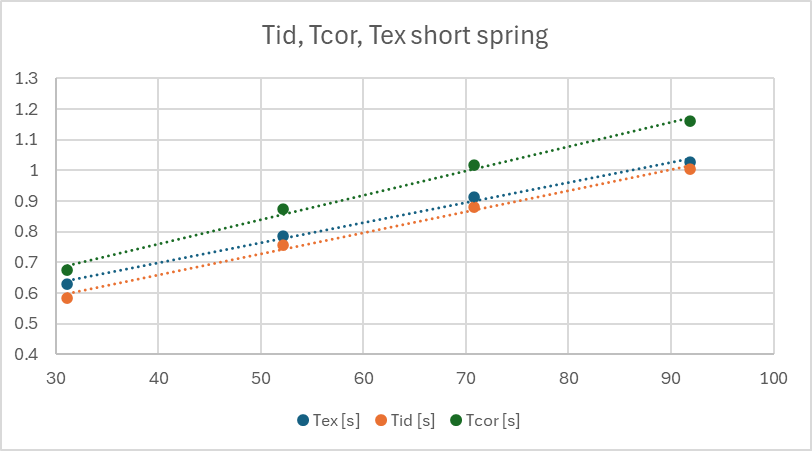
\includegraphics[width = 0.9\textwidth]{Shortspring_period.png}
    \caption{$T_{ex}, T_{id}, T_{cor}$ in terms of mass for the short spring}
\end{figure}
\begin{figure}[!h]
    \centering
    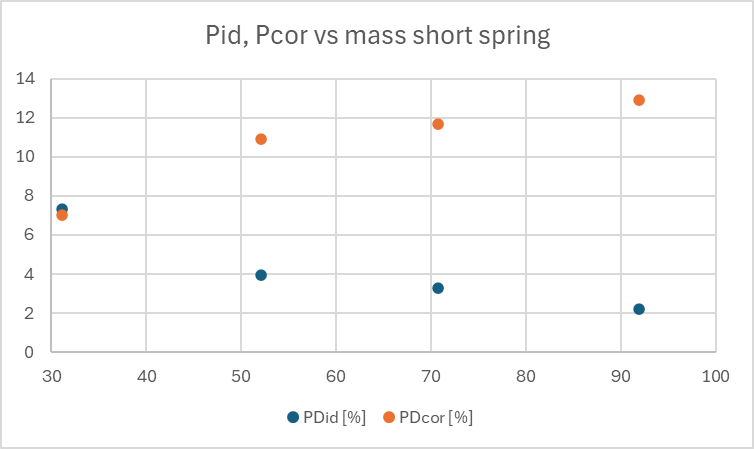
\includegraphics[width = 0.9\textwidth]{Shortspring_deviation.png}
    \caption{$PD_{id}, PD_{cor}$ in terms of mass for the short spring}
\end{figure}
\begin{figure}[!h]
    \centering
    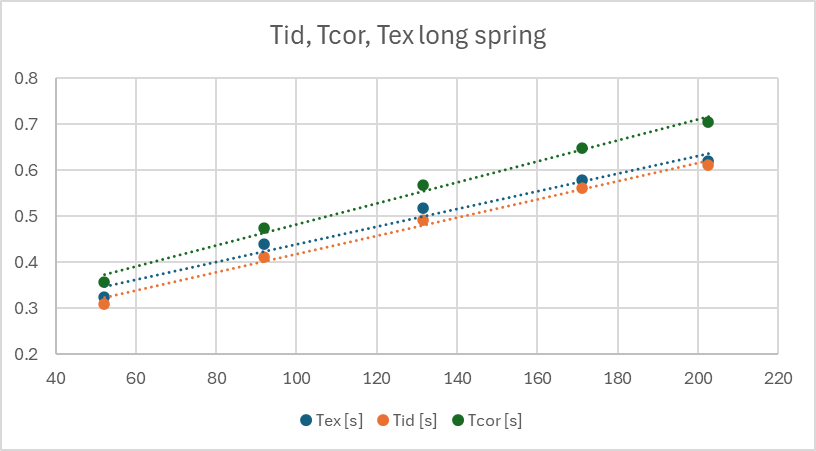
\includegraphics[width = 0.9\textwidth]{Longspring_period.png}
    \caption{$T_{ex}, T_{id}, T_{cor}$ in terms of mass for the long spring}
\end{figure}
\begin{figure}[!h]
    \centering
    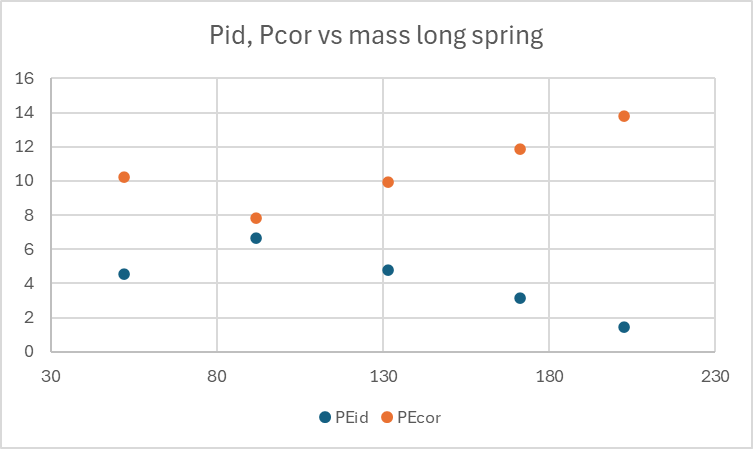
\includegraphics[width = 0.9\textwidth]{Longspring_deviation.png}
    \caption{$PD_{id}, PD_{cor}$ in terms of mass for the long spring}
\end{figure}
\newpage
\subsection{Calculations}
Using the forth data point of table \ref{tab:3} these calculations are done for
the short spring.
\par
\textbf{Calculating the experimental period:}
\\
From the data, $T_{ex}$ is
\[T_{ex} = \frac{1}{30} \cdot \frac{30.82 + 30.92 + 30.7}{3} = 1.03\unit{s}\]
\par
\textbf{Ideal period of oscillation:}
\\
From equation \ref{eq:6} the ideal oscillation period is
\[ T_{id} = 2 \pi \sqrt{\frac{91.9 \cdot 10^{-3}\unit{kg}}{3.53 \unit{kg
s^{-2}}}} = 1.01\unit{s}\]
\par
\textbf{Corrected period of oscillation:}
\\
From equation \ref{eq:7} the period of one oscillation with the corrected weight
is 
\[ T_{cor} = 2 \pi \sqrt{\frac{91.9 \cdot 10^{-3}\unit{kg} + \frac{91.9\cdot
10^{-3}\unit{kg}}{3}}{3.53 \unit{kgs^{-2}}}} = 1.16\unit{s}\]
\par
\textbf{Ideal and corrected percent deviation:}\\
The deviation in both cases is calculated using the following formula
\begin{equation}
    PD = \frac{T_{ex} - T}{T}
\end{equation}
where T is either the ideal or corrected period.\\
Therefore, 
\begin{gather*}
    PD_{id} = \frac{1.03\unit{s} - 1.01\unit{s}}{1.01\unit{s}}\cdot100\unit{\%} = 2.23\unit{\%}\\
    PD_{cor} = \frac{1.03\unit{s} - 1.16\unit{s}}{1.16\unit{s}}~100\unit{\%} = 12.9\unit{\%}
\end{gather*}
\subsubsection{Error calculations}
\textbf{Error in the period of one theoretical oscillation:}\\
Using equation \ref{eq:10} the error in the theoretical period is 
\begin{gather*}
    \Delta T_{id} = \left| 1.01\unit{s} \right| \cdot \sqrt{\left(\frac{0.01 \cdot 10^{-3}\unit{kg}}{91.9 \cdot 10^{-3}\unit{kg}}\right)^2 + \left(\frac{0.04 \unit{kg s^{-2}}}{3.52\unit{kg s^{-2}}}\right)^2} \approx 0.075\unit{s}\\
    \Delta T_{cor} \approx 0.086\unit{s}
\end{gather*}
\par
\textbf{Error in the experimental period value:}\\
Using equations \ref{eq:12}, \ref{eq:13}, \ref{eq:14} the error for the
experimental value is calculated using the standard deviation of the mean. The
values gathered from the forth mass in table \ref{tab:3} are
\begin{gather*}
    s = \pm0.0037\unit{s}\\
    s_m = \pm0.0022\unit{s}\\
    \Delta T_{ex} = \pm 0.0064\unit{s}
\end{gather*}
\par
Tables 5 and 6 contain all the error values for the second experiment.
\begin{table}[!h]
    \centering
    \caption{Error values for the short spring measurements}
    \begin{tabular}{|c|c|c|c|c|c|} 
    \hline
    $m~[10^{-3}\unit{kg}]$ & standard deviation of T [s] & $s_m$ [s] & $\Delta T_{ex}\unit{[s]}$ & $\Delta T_{id}\unit{[s]}$ &
    $\Delta T_{cor}\unit{[s]}$  \\ 
    \hline
    31.14            & 0.0052                     & 0.003                           & 0.009 & 0.043 & 0.050   \\ 
    \hline
    52.14            & 0.003                    & 0.002                           & 0.005 & 0.056 & 0.064   \\ 
    \hline
    70.8             & 0.005                    & 0.003                           & 0.009 & 0.065 & 0.075   \\ 
    \hline
    91.9             & 0.004                    & 0.002                            & 0.006  & 0.074 & 0.085   \\
    \hline
    \end{tabular}
    \end{table}
    \begin{table}[!h]
        \centering
        \caption{Error values for the long spring measurements}
        \begin{tabular}{|c|c|c|c|c|c|} 
        \hline
        $m~[10^{-3}\unit{kg}]$ & standard deviation of T [s]& $s_m\unit{[s]}$ &
        $\Delta T_{ex}\unit{[s]}$     & $\Delta T_{id}\unit{[s]}$     & $\Delta
        T_{cor}\unit{[s]}$     \\ 
        \hline
        52.14     & 0.001                & 0.0008                       & 0.0024 & 0.0228 & 0.0264  \\ 
        \hline
        91.9      & 0.0076                & 0.0044                       & 0.0132 & 0.0304 & 0.0351  \\ 
        \hline
        131.46    & 0.0036                & 0.0021                       & 0.0062 & 0.0363   & 0.0419  \\ 
        \hline
        171.12    & 0.0072                & 0.0042                       & 0.0125  & 0.0414 & 0.0478  \\ 
        \hline
        202.64    & 0.0021                & 0.0012                       & 0.0036 & 0.0451 & 0.0520  \\
        \hline
        \end{tabular}
        \end{table}
\section{Discussion period}
The ideal period $T_{id}$ depends on the mass according to the formula where k is the spring constant. This indicates that rather than increasing linearly, the period rises with the square root of the mass. Plotting Tid against m results in a curve that flattens off as mass increases.
\par
The square root relationship predicted the shape of the curves we saw during the experiment. Small variations from the anticipated shape were probably caused by friction, a small amount of air resistance, or minor spring flaws. Although these problems are difficult to eliminate in real-world research, they don't significantly affect the general patterns.
\par
The mass determines the difference between $T_{cor}$ and Tid. The adjustment has a greater effect when the mass is smaller since the mass of the spring makes up a larger portion of the entire system. The spring's contribution decreases with increasing mass, and the difference between $T_{cor}$ and Tid narrows. This indicates that while working with lighter loads, the adjustment is more important.
\par
The percentage gap between the experimental data and the theoretical values decreases with increasing mass. At larger masses, measurement errors, random errors, and other little problems have less of an impact on the overall behavior of the system. Consequently, a larger mass leads to a higher agreement between the theoretical and experimental values.
\par
We could use instruments like a digital caliper to measure the spring's
displacement under various forces, which would decrease measurement errors and
provide a more precise estimate for k. We could use more accurate timing
devices, make sure the spring doesn't move sideways, and perform repeated
measurements to average out any random changes in order to determine the
vibration period more accurately. These enhancements would increase the accuracy
of our findings and bring them closer to the theoretical forecasts. 
\section{Conclusion}
In conclusion, the experiment shows that the square root dependency indicated by
Hooke's rule is followed in the relationship between mass and period.
Specifically, when dealing with smaller masses, the corrected period $T_{cor}$
matched the experimental data far better than the ideal period $T_{id}$. Differences
between theoretical and practical data were minor which are within the
anticipated error range. Also, outcomes of the experiment were parallel with
predictions and similar studies. 
\section{Bibliography}
\bibliographystyle{IEEEtran}
\bibliography{refrences.bib}
\end{justify}
\includepdf[pages = {10}]{template.pdf}
\end{document}